\chapter{Synthèse de circuits, Quine Mc.Cluskey}
\section{Synthèse des circuits à partir de spécification verbales}
\paragraph{Spécification formelle} Description complète, précise et non-ambiguë de toutes les propriétés d'un système (TdV, K-Map etc.).
\paragraph{Combinatoire} Les sorties du système ne dépendent que des entrées.\\

Si le problème \textbf{est combinatoire}, alors on peut appliquer tout ce qui a été vu jusqu'à présent.\\
N.B. : commencer par déterminer le nombre d'entrées et de sorties
\section{Additionneurs re-visités}
On souhaite réaliser un circuit additionneur de deux mots A et B codés sur 4 bits (peut généraliser pour $n$ bits).\\
deux solutions s'offrent à nous:
\begin{itemize}
	\item Mimer le principe d'addition bit à bit (séquence de calcul dans le temps)
	\item Anticiper le report pour un certain nombre de bits (considérer le problème comme combinatoire)
\end{itemize}
\subsection{Addition bit à bit}
L'addition est faite grâce à:
\begin{itemize}
	\item un 1/2 additionneur (deux opérantes d'un bit, deux bits d'entrées)
	\item $(n-1)\times$ additionneur complet (deux opérantes d'un bit + un bit de report d'une étage précédent, trois bits d'entrées)
\end{itemize}
\begin{minipage}{.45\textwidth}
	\begin{figure}[H]
		\centering
		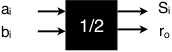
\includegraphics[width=.6\textwidth]{ch5/image1}
	\end{figure}
\end{minipage}
\begin{minipage}{.55\textwidth}
	\begin{figure}[H]
		\centering
		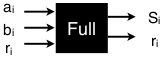
\includegraphics[width=.48\textwidth]{ch5/image2}
	\end{figure}
\end{minipage}
\begin{minipage}[t]{.25\textwidth}
	\begin{table}[H]
		\centering
		$\begin{array}{|c|c|c|c}
			\cline{1-3}
			S_i & 0 & 1 & b_i\\
			\cline{1-3}
			0 & 0 & 1 & \\
			\cline{1-3}
			1 & 1 & 0 & \\
			\cline{1-3}
			\multicolumn{1}{c}{a_i} & \multicolumn{1}{c}{ } & \multicolumn{1}{c}{ }		
		\end{array}$
		\begin{align*}
			S_i &=a_i'b_i+a_ib_i'\\
			&= a_i  \oplus b_i
		\end{align*} 
	\end{table}

\end{minipage}
\begin{minipage}[t]{.2\textwidth}
	\begin{table}[H]
		\centering
		$\begin{array}{|c|c|c|c}
			\cline{1-3}
			r_0 & 0 & 1 & b_i\\
			\cline{1-3}
			0 & 0 & 0 & \\
			\cline{1-3}
			1 & 0 & 1 & \\
			\cline{1-3}
			\multicolumn{1}{c}{a_i} & \multicolumn{1}{c}{ } & \multicolumn{1}{c}{ }		
		\end{array}$
		\begin{equation*}
			r_0 = a_ib_i
		\end{equation*} 
	\end{table}
\end{minipage}
\begin{minipage}[t]{.3\textwidth}
	\begin{table}[H]
		\centering
		$\begin{array}{|c|c|c|c|c|c}
			\cline{1-5}
			S & 00 & 01 & 11 & 10 & a_ib_i\\
			\cline{1-5}
			0 & 0 & 1 & 0 & 1 & \\
			\cline{1-5}
			1 & 1 & 0 & 1 & 0 & \\
			\cline{1-5}
			\multicolumn{1}{c}{r_i} & \multicolumn{1}{c}{ } & \multicolumn{1}{c}{ } & \multicolumn{1}{c}{ } & \multicolumn{1}{c}{ } & \multicolumn{1}{c}{ } 	
		\end{array}$
		\begin{equation*}
			S = a_i\oplus b_i\oplus r_i
			\end{equation*} 
	\end{table}
\end{minipage}
\begin{minipage}[t]{.3\textwidth}
	\begin{table}[H]
		\centering
		$\begin{array}{|c|c|c|c|c|c}
			\cline{1-5}
			r & 00 & 01 & 11 & 10 & a_ib_i\\
			\cline{1-5}
			0 & 0 & 0 & 1 & 0 & \\
			\cline{1-5}
			1 & 0 & 1 & 1 & 1 & \\
			\cline{1-5}
			\multicolumn{1}{c}{r_i} & \multicolumn{1}{c}{ } & \multicolumn{1}{c}{ } & \multicolumn{1}{c}{ } & \multicolumn{1}{c}{ } & \multicolumn{1}{c}{ } 	
		\end{array}$
		\begin{equation*}
			r = a_ib_i+r_ib_i+r_ia_i
		\end{equation*} 
	\end{table}
\end{minipage}
Ainsi, pour un additionneur complet sur 4 bits:
\begin{figure}[H]
	\centering
	
\includegraphics[scale=0.7]{ch5/image3}
\end{figure}
Le problème de ce système est la propagation du report entre les étages: le résultat final sera obtenu après la propagation du report à travers tous les étages de l’additionneur ($n$-délais).
\subsection{Additionneur \textit{Carry Look Ahead} (CLA)}

\section{Encodeurs de priorité}

\section{Simplification des fonctions : Méthode Quine-Mc.Cluskey}
La méthode de Quine-Mc.Cluskey est:
\begin{itemize}
	\item méthode systématique, analysant toutes les possibilités de regroupement. 
	\item utilisée pour un grand nombre de variables
	\item garantit la meilleure solution
	\item facilement programmable
\end{itemize}
Elle se base sur 2 étapes:
\begin{enumerate}
	\item Recherche des implicants premiers (phase d'\textbf{analyse}) par la \textbf{méthode des tris successifs}
	\item Couverture de la fonction (phase de \textbf{synthèse}) par un choix des implicants premiers
\end{enumerate}
\subsection{Étape 1: Analyse}
\iffalse
Elle consiste en 11 étapes:
\begin{enumerate}
	\item Pour une fonction $f$ de $n$ variables, on construit $m$ groupements de \textbf{tous les mintermes} de la fonction
	\item Dans chaque groupement des mintermes (noté $G_i$)
	\begin{itemize}
		\item $i$ variables qui valent 1
		\item $(n-i)$ variables qui valent 0
	\end{itemize}
	\item On compare chaque minterme de $G_i$ avec \textbf{TOUS} les mintermes appartenant à $G_{i+1}$ en termes de la distance de Hamming ($\forall i$)
	\item Si la distance de Hamming entre 2 mintermes $=1$, on note \textbf{l'appariement} entre les 2:
	\begin{equation}
		\left.
			\begin{array}{r}
				000\\
				010
			\end{array}
		\right\}\Rightarrow 0\text{-}0
	\end{equation}
	\item Tous les appariements de $G_i$ et $G_{i+1}$ sont écrits dans un nouveau groupement, noté $G_i'$
	\item Après une première passe, il y a donc au moins $m-1$ groupements $G_i'$
	\item Lors de l'appariement de $G_i$ et $G_{i+1}$, il est possible qu'un minterme n'ait pas été regroupé avec d'autres
	\begin{itemize}
		\item c'est un impliquant premier (n-cube de taille 1 à ce stade)
		\item On les note $IP_k$ dans l'ordre dans lequel ils apparaissent
	\end{itemize}
	\item L'ensemble $G_i'$ constitue 
\end{enumerate}
\fi